\section{Density-Based}
    Il Density-Based Clustering funziona rilevando le aree in cui i punti sono concentrati e dove sono separati da aree vuote o sparse.
    I punti che non fanno parte di un cluster vengono etichettati come rumore.
    \\[1\baselineskip]
    Funziona bene anche il il clustering temporale: i valori delle feature temporali dei punti possono essere utilizzate per trovare gruppi di punti che si raggruppano insieme nello spazio e nel tempo.
    \\[1\baselineskip]

    \subsection{DBSCAN}
        Il $\textbf{Density-Based Spatial Clustering of Applications}$\\$\textbf{with Noise}$ (DBSCAN) utilizza una distanza specificata ($\epsilon$) per separare i cluster densi dal rumore più sparso.
        \\[1\baselineskip]
        L'algoritmo DBSCAN è il metodo di clustering più veloce, ma è appropriato solo se viene già definita una distanza di ricerca e che funzioni bene per tutti i potenziali cluster.
        Ciò richiede che tutti i cluster significativi abbiano densità simili.
        \\[1\baselineskip]
        L'algoritmo utilizza il concetto di raggiungibilità della densità ($\textbf{density reachability}$) e connettività della densità\\ ($\textbf{density connectivity}$):
            \begin{itemize}
                \item $\textbf{Density Reachability}:$ si dice che un punto $p$ sia "density reachable" da un punto $q$ se il punto $p$ si trova entro una distanza $\epsilon$ dal punto $q$ e $q$ ha un numero sufficiente di punti nei suoi vicini che sono a distanza $\epsilon$.
                    \begin{figure}[h]
                        \centering
                        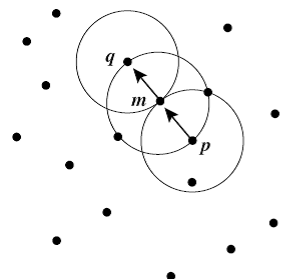
\includegraphics[width = 5cm, height = 5cm]{density-reachability.png}
                    \end{figure}
                \item $\textbf{Density Connectivity}:$ si dice che un punto $p$ e $q$ sono "density connected" se esiste un punto $r$ che ha un numero sufficiente di punti nei suoi vicini ed entrambi i punti $p$ e $q$ sono all'interno della distanza $\epsilon$.
                    \\
                    Per esempio, se $q$ è vicino di $r$, $r$ è vicino di $s$, $s$ è vicino di $t$ che a sua volta è vicino di $p$, allora anche $q$ è vicino di $p$.
                    \begin{figure}[h]
                        \centering
                        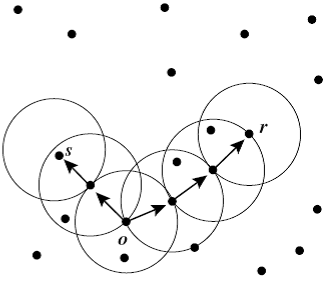
\includegraphics[width = 5cm, height = 5cm]{density-connected.png}
                    \end{figure}
            \end{itemize}

        \subsubsection{Algoritmo}
            Siano $X = {x_{1}, x_{2}, \ldots, x_{n}}$ l'insieme dei punti.
            DBSCAN richiede due parametri: $\epsilon$ e il numero minimo di punti richiesti per formare un cluster ($MinPts$).
            \\[1\baselineskip]
            $\textbf{Nota:}$ I parametri $\epsilon$ e $MinPts$ sono degli iperparametri che devono essere decisi prima del lancio dell'algoritmo.

            \begin{enumerate}
                \item Inizia con un punto di partenza arbitrario che non è stato visitato;
                \item Estrae l'intorno di questo punto usando $\epsilon$ (tutti i punti che si trovano all'interno della distanza $\epsilon$ sono i vicini);
                \item Se ci sono abbastanza vicini attorno a questo punto, il processo di raggruppamento inizia e il punto viene contrassegnato come visitato, altrimenti questo punto viene etichettato come rumore;
                    \\[0.5\baselineskip]
                    $\textbf{Nota:}$ in seguito questo punto può diventare parte del cluster.
                \item Se scopre che un punto fa parte del cluster, allora anche il suo intorno $\epsilon$ è parte del cluster e gli steps dal punto (2) vengono ripetuti per tutti i punti dell'intorno $\epsilon$.
                    \\
                    Questo viene ripetuto finché non vengono determinati tutti i punti nel cluster;
                \item Un nuovo punto non ancora visitato viene preso ed elaborato, portando alla scoperta di un ulteriore cluster o etichettandolo come rumore;
                \item Continuo questo processo finché tutti i punti non vengono contrassegnati come visitati.
            \end{enumerate}

        \subsubsection{Vantaggi}
            \begin{itemize}
                \item Non richiede la specificazione a priori del numero di cluster;
                \item È in grado di identificare rumore durante il clustering;
                \item È in grado di trovare cluster di dimensioni e forma arbitrarie.
            \end{itemize}

        \subsubsection{Svantaggi}
            \begin{itemize}
                \item Fallisce in caso di cluster a densità variabile;
            \end{itemize}

        \begin{figure}[h]
            \caption{Esempio di risultato del DBSCAN}
            \centering
            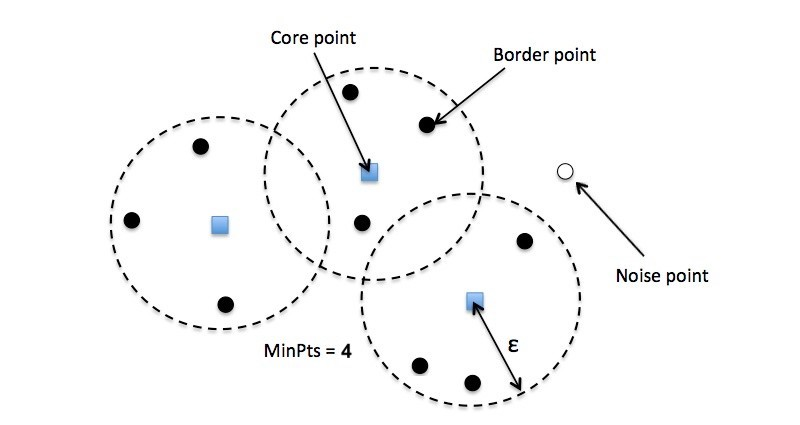
\includegraphics[width = 10cm]{dbscan-example.jpeg}
        \end{figure}

\clearpage